\documentclass[9pt,twocolumn,twoside,lineno]{pnas-new}
%% \documentclass[9pt,twocolumn,twoside]{pnas-new}

\templatetype{pnasresearcharticle} % Choose template 
\title{Demographic Perspectives on the Mortality of Covid-19 and Other
  Epidemics}
\date{June 1, 2020}

\author[a,1]{Joshua R. Goldstein}
\author[a,1,2]{Ronald D. Lee}

\affil[a]{Department of Demography, UC Berkeley}

% \author{Joshua R. Goldstein \and Ronald D. Lee}
\leadauthor{Goldstein}

\significancestatement{What would a hypothetical one million
  U.S. deaths in the Covid-19 epidemic mean for mortality of
  individuals at the population level?  Life expectancy for 2020 would
  drop by 2.9 years. Those dying would lose an average of 11.7 years
  of expected remaining life, while for the general population the
  loss of remaining life would be .2 years for elders (at age 80)
  and much less at younger ages. Mortality per person would be less
  than the Spanish Flu, but closer to the opioid and HIV/AIDS
  epidemics, while far more concentrated in time. The standard
  valuation of averting 1.75 million deaths would be many trillions of
  dollars.}

% \authorcontributions{Please provide details of author contributions here.}
% \authordeclaration{Please declare any conflict of interest here.}
\equalauthors{\textsuperscript{1}J.G. and R.L. contributed equally to this work.}
\correspondingauthor{\textsuperscript{2}To whom correspondence should be addressed. E-mail: rlee@demog.berkeley.edu}

\keywords{coronavirus $|$ covid-19 $|$ epidemic $|$ mortality $|$ demography $|$ life
expectancy}

\begin{abstract}
  To put estimates of Covid-19 mortality into perspective, we estimate
  age-specific mortality for an epidemic claiming for illustrative
  purposes one million U.S. lives, with results approximately scalable
  over a broad range of deaths. We calculate the impact on period life
  expectancy (down 2.94 years) and remaining life-years (11.7 years
  per death).  Avoiding 1.75 million deaths or 20.5 trillion
  person-years of life lost would be valued at 10.2 to 17.5 trillion
  dollars. The age-patterns of Covid-19 mortality in other countries
  are quite similar and increase at rates close to each country's rate
  for all-cause mortality. The scenario of one million Covid-19 deaths
  is similar in scale to the decades-long HIV/AIDS and opioid-overdose
  epidemics but considerably smaller than the Spanish Flu of
  1918. Unlike HIV/AIDS and opioid epidemics, the Covid-19 deaths are
  concentrated in a period of months rather than spread out over
  decades.
\end{abstract}


\begin{document}
\maketitle
\thispagestyle{firststyle}
\ifthenelse{\boolean{shortarticle}}{\ifthenelse{\boolean{singlecolumn}}{\abscontentformatted}{\abscontent}}{}
 

\dropcap{A}s we write, societies around the world are struggling to
protect their populations from the Covid-19 pandemic. Both citizens
and policy makers are trying to make sense of the magnitude of the
crisis and the lives that it threatens.

In this paper, we provide several different ways to think about the
mortality of the epidemic. It is possible to portray the death toll in
a way that feels overwhelmingly large, but it is also possible to
describe it in a way that makes the epidemic mortality seem almost
negligible. Our view is that Covid-19 should be seen as an extremely
large mortality threat. By most measures, the threat of the current
epidemic is smaller in scale than the Spanish Flu, but Covid-19
mortality could in a matter of months be equal in overall
magnitude to the decade's long HIV and opioid epidemics.

Our intention here is not to provide new forecasts of Covid-19
mortality. Instead, we combine existing projections with observations
to date about the age pattern of mortality, producing an estimated
age-profile of Covid-19 mortality. This age-profile, which can be
scaled up or down, enables estimation of the epidemic’s impact on
period life expectancy and loss of person-years of life at a
population scale, as well as comparison with past epidemics.

A further contribution of the paper is to show that the age-pattern of
deaths, when appropriately adjusted, is quite similar across a
wide-range of countries and stages of the epidemic. Indeed, the
increase in mortality by age from Covid-19 strongly resembles
the age-pattern of all-cause mortality. Whereas all-cause mortality
tends to follow Gompertz's law, increasing exponentially at a constant
rate of about 10\% per year of age, Covid-19 mortality increases at
about 11\% per year of age. There is some variation across
populations, but this too seems to echo background mortality. 
The age-profile of Covid-19 mortality may change over time, as
treatment becomes more (or less) available. However, the age-gradient
we see to date suggests that the risk factors for Covid-19 are similar
to those for all causes of death.

Epidemiological models for the United States are predicting from
118,000 to 143,000 Covid-19 deaths by June 27, with Youyang Gu
projecting 187,000 deaths by September 1 \cite{cdc:2020}. The prospect
of subsequent waves in the Fall and afterwards is uncertain. Earlier
projections of epidemic mortality suggested that deaths could total
more than 2 million if nothing were done to slow the spread of the
novel coronavirus \cite{ferguson:2020}.  For illustrative purposes we
use an intermediate scenario of 1 million deaths in 2020 due directly
to Covid-19 across all waves, at times comparing it to a lower
scenario of 250,000 and higher of 2 million. The metrics we produce
scale approximately proportionately with the number of deaths, so readers
can translate our results under different mortality scenarios.

The age-pattern we use in this paper does not include the indirect
increase in deaths as healthcare systems are overwhelmed, or the
long-term effect of infection on the mortality of survivors. It also
does not take into account any potential lowering of mortality, for
example, from decreased air pollution, traffic accidents and
consumption of alcohol resulting from the economic slowdown. These
effects may be important, but the age pattern of these changes might
be quite different.

As we describe below, the most commonly used measure of mortality,
life expectancy at birth, is not a good measure of transitory
mortality shocks. Other measures, including the crude death rate,
age-specific mortality, and the loss of remaining person years of life
together give a better summary of the magnitude of epidemic
deaths. These perspectives allow us to compare mortality impacts over
time and across populations. They also allow policy makers to make
more informed judgments about the valuation of saved lives.

\section*{Mortality Measures}

The most direct indicator of mortality is the number of deaths. This
count is often given relative to population size. In the absence of
the epidemic, recent levels of mortality suggest there would have been
about 3 million deaths in the U.S. population of 330 million,
giving a crude death rate of about 9.1 per thousand.

\begin{figure*}[h]%[tbhp]
\centering
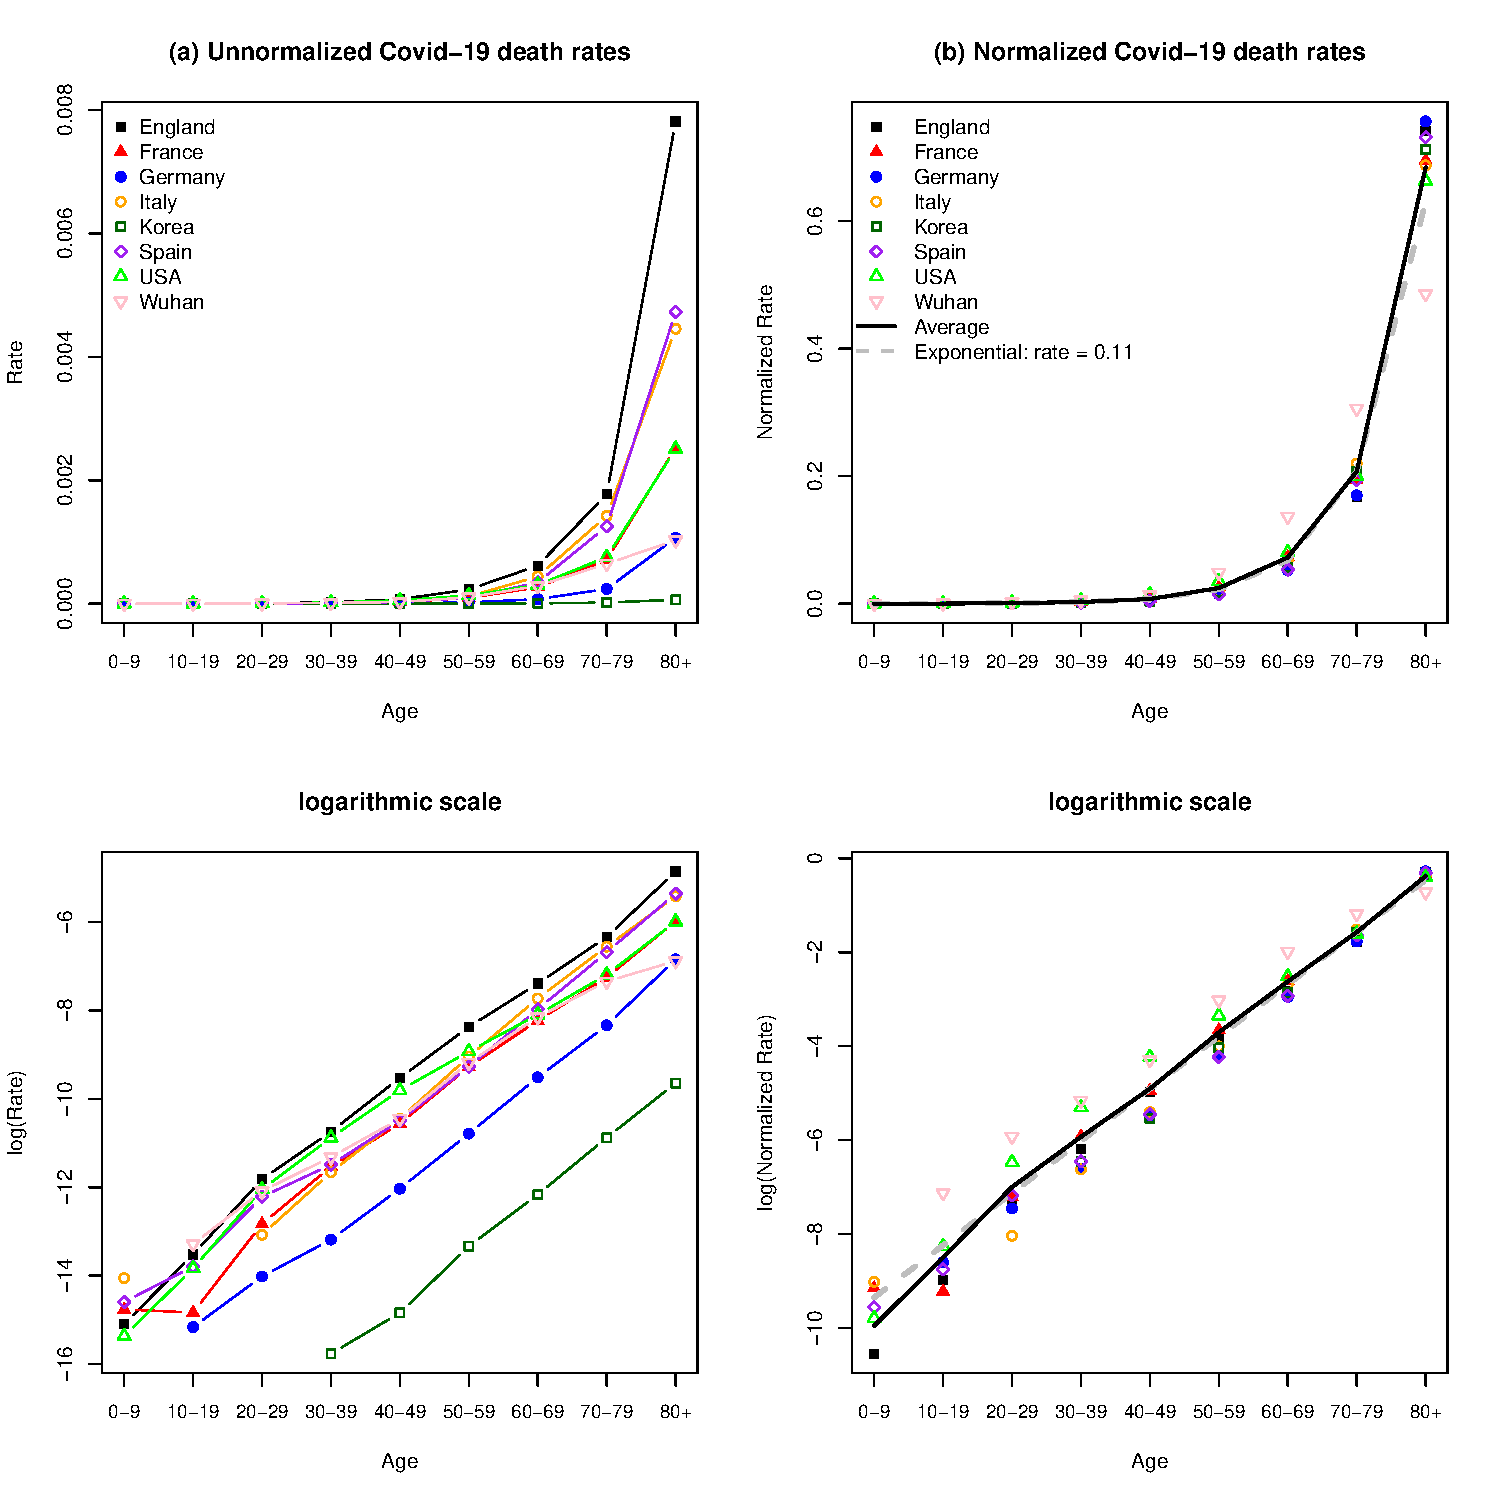
\includegraphics[width=.8\linewidth]{fig1_age_specific_covid_rates}
\caption{Similar Age Pattern of Covid-19 mortality by Region. (a)
  Unnormalized age-specific mortality, calculated as the ratio of
  deaths by age to population by age. The levels should not be
  interpreted as reflecting real differences in mortality because of
  unaccounted variation in time scale, stage of the epidemic, and the
  extent of spread within the region (b) Normalized rates, dividing
  each region's rates by the sum of these rates, allow comparison of
  the age pattern. The average is calculated across all
  regions. Exponential increase at a rate of 0.11 is plotted to
  intersect the average in the age group 70-79. Lower panels show the
  same data as upper panels but in logarithmic scale. (Sources, see
  text and materials and methods \ref{sec:rate}.)}
\label{fig:asmr}
\end{figure*}

An additional 1 million deaths from Covid-19 would increase the total
annual deaths to 4 million, raising the crude death rate to about
12.1/1000 (or to 9.9/1000 if there were 250,000 Covid-19 deaths). The
increased risk to the average person is small in absolute size but
large in relative terms, with a proportional increase of a 1/3 for 1
million deaths and 1/12 for 250,000 deaths.  Epidemic mortality in a
given region may be compressed into a small portion of the year: if
most of the deaths occurred within a three month period, the daily
risk of mortality implied by an additional million deaths during this
time would be more than double its normal level.

The epidemic is much more dangerous for the elderly than the
young. The most commonly reported age-specific measure is the ``case
fatality rate'' (CFR), which is the ratio of Covid-19 deaths to
diagnosed cases by age. There are challenges in the classification and
reporting of Covid-19 deaths, in particular whether the coverage is
restricted to hospitals or also includes deaths occurring at home or in
nursing homes. But the bigger problem in relying on the CFR is the
measurement of the denominator, the number of cases. Cases can be
defined within hospital systems, or within a testing regime, but
neither approach is a reliable indicator of the actual number of
infected individuals at the population level.


As an alternative, we estimate cause-specific mortality rates by age,
using the counts in age groups of the entire population, focusing on
the relative risk by age, rather than the overall level. We use
compiled age specific death data from countries – China
\cite{novel:2020}, S. Korea, Italy, Spain, France, Germany, England
and Wales, and the United States \cite{ined:2020}.\footnote{For China,
we use the population age distribution of Hubei because 840 of the
1,023 deaths in Chinese data were in Hubei. We thank Prof. Yi Zhou
for these calculations.} Our approach does not require that the
counts of deaths have the same level of completeness across countries,
which vary both in the definitions they use and in the stage of the
epidemic for which we observe them. But we do assume that the
age-distributions of reported Covid-19 deaths are accurate.

For each country, we calculate (unnormalized) age-specific death rates
(ASDR) using reported Covid-19 deaths by age and the population by
age, typically for the nation as a whole (See Figure \ref{fig:asmr}(a)). We
standardize mortality across countries for the open age interval (80+)
to account for differences in the population age distribution of the
elderly in different countries (see materials and methods \ref{sec:indirect}).
Since the epidemic may be concentrated in one part of the country, and since
some countries may be at earlier stages with fewer reported deaths,
these ASDR may be extremely low in some countries and much higher in
others, which does not necessarily signal a more or less severe
epidemic and should not be so interpreted. Instead, we believe that
the most reliable information is the shape or pattern by age of death
rates, abstracting from the level.  To make the age-pattern comparable
across populations, we normalize each country's rates by dividing by
the sum of the rates, so that the normalized rates sum to 1.0.  We can
see that the age-patterns are quite similar across the 8
countries. (See Figure \ref{fig:asmr}(b)).


It is evident from Figure \ref{fig:asmr} that Covid-19 mortality risk
is many times higher for the old than the young, and indeed the vast
majority of Covid-19 deaths are of older people. But the same is true
for all-cause mortality -- the vast majority of deaths are of the
elderly. About 70\% of all U.S. Covid-19 deaths are to age 70 or
above, somewhat above the 64\% for normal mortality. In fact, the
age-distribution of deaths attributed to Covid-19 is quite similar to
that of all-cause mortality, which tends to increase by about 10\%
every year of age after age 30. Figure \ref{fig:asmr}(b) shows that in
South Korea, Italy, France, Germany, the England and Wales, and Spain,
virus-attributed mortality rates rise by about 12\% per year, while
the United States and Wuhan show a slower rate of increase (about
9.5\% per year of age).

At ages under 40, Covid-19 mortality risk is low, but so is mortality
from other causes. It appears in the lower panel of Figure
\ref{fig:asmr}(b) that average mortality below 20 or 30 is less than
would be predicted from the exponential pattern of mortality at older
ages. However, the number of cases is so small that we are hesitant to
draw a conclusion before more data become available.

There also appears to be a relationship between the age-distribution
of Covid-19 mortality and that of all-cause mortality that holds
across countries. Figure \ref{fig:gompertz} shows the exponential rate
of increase in mortality by age for all-causes and for Covid-19, for
countries in the Human Mortality Database. The rate of increase of
all-cause mortality varies from country to country around a central
value of about .10, higher than the .086 for the United States. The
smaller rate of increase in the United States is due to unusually high
mortality at younger ages, not advantages at older ages, and has been
used as an indirect indicator of the inequality of health status of
the population \cite{edwards:2005,aburto:2020}.  From this small
number of countries, at least, it appears that Covid-19 may be echoing
the same factors as all-cause mortality, suggesting that there may be
a relationship between the level of health inequality within
populations and the age pattern of Covid-19 mortality.


\begin{figure}[h]%[tbhp]
\centering
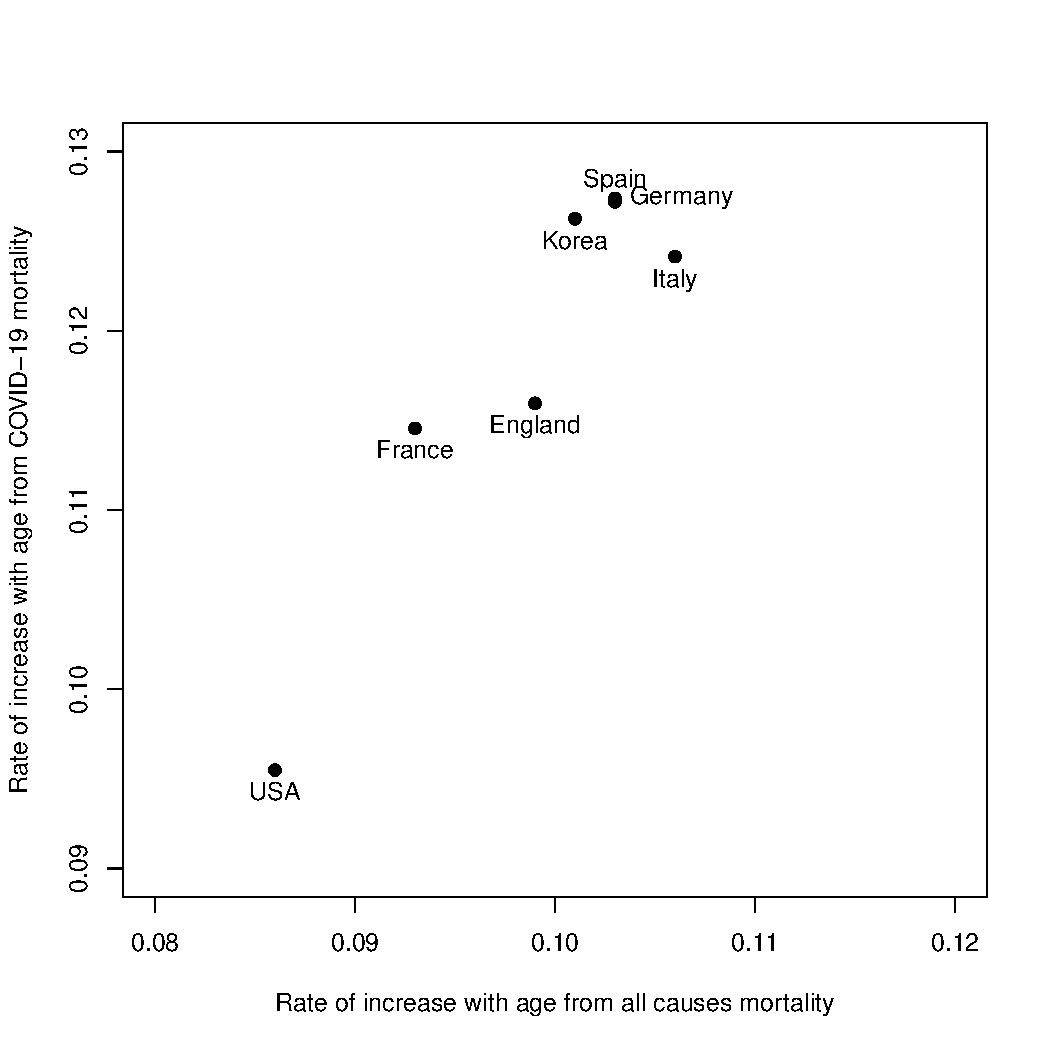
\includegraphics[width=.8\linewidth]{fig2_gompertz_scatter}
\caption{The relationship between exponential rates of increase with age of
  all-cause mortality and Covid-19 mortality for countries in the
  Human Mortality Database. (Note: exponential rates are calculated
  from age groups 45-49 to 85-89 for all-cause mortality and ages
  40-49 to 80$+$ for Covid-19 mortality, assuming 40-year ranges for
  both.)}
\label{fig:gompertz}
\end{figure}



All the above results are for sexes combined mortality, the approach
we take throughout this study. As an aside, however, analysis of
Covid-19 mortality by sex in the United States finds a steeper rate of
increase for females above age 35 (just above .10 per year) than males
(just below .09), so the ratio of male to female Covid-19 death rates
which is 1.44 from 35-54 declines thereafter across ten year age
groups to 1.37, 1.34, 1.26, and finally 1.12 for 85+. Despite the
widespread reporting of higher Covid-19 mortality to males, the
relative risk of males to females is actually lower for Covid-19 than
for all-cause mortality in the United States in 2017 \cite{HMD}.  

\section*{Epidemic mortality risk as temporary aging}



We can translate the elevated risk of mortality during an epidemic
into a measure of ``temporary aging.'' This measure expresses the
increased risk of an individual during the months of the epidemic in
terms of the age of someone with equivalent mortality during normal,
non-epidemic times. If $R$ is the ratio of mortality during the
epidemic to normal mortality and $\beta$ is the exponential rate of
increase of all-cause mortality with age, then the years of implied
``temporary aging'' will be $\log(R)/\beta$. For example, if there
were 1 million Covid-19 deaths within a 3 months period when only
750,000 deaths would normally occur, and if $\beta = 0.10$, then the
years of temporary aging would be $\log(1.75/0.75)/.1 = 8.5$. This
same effect applies across the range of ages when mortality is
increasing at this rate, approximately from ages 30 to 85.


\begin{table}[h]%[tbhp]
\centering
\caption{Years of ``temporary aging'' for hypothetical epidemics with
  mortality concentrated in a three month period.}
\label{tbl:aging}
\begin{tabular}{rr}
  Deaths & Temporary Aging \\
  (1,000s) & (years) \\
\midrule
  2,000 & 13.0 \\
  1,000 & 8.5 \\
  500  & 5.1 \\
  250  & 2.9 \\
  125 & 1.5 \\ 
\bottomrule
\end{tabular}

\addtabletext{For example, during a U.S. epidemic with 1 million
  deaths, an 80 year old would be exposed the normal mortality risk of
  an 88.5 year old. Note: estimates assume a 10\% rate of mortality
  increase with each year of age.}
\end{table}


Table \ref{tbl:aging} shows such calculations for different
epidemiological forecasts for the United States in terms of temporary
aging, assuming a 3 month window of epidemic mortality and
$\beta = 0.10$. We provide a range from as low as 125,000 -- the
midrange of the CDC (2020) summarized projections to June 27 -- to a
high of 2 million, a bit less than the estimate of an uncontrolled
epidemic \cite{ferguson:2020}. The estimates in Table \ref{tbl:aging}
tell us that a scenario of 1 million Covid-19 deaths over the course
of 3 months exposes a 30 year old to the risks of a 38.5 year old in
normal times and exposes an 80 year old to the risks of an 88.5 year
old in normal times. The same number of years of temporary aging,
however, pose different absolute increases in risk. For the 30 year
old, the absolute increase in mortality would be small, but for the 80
year old it would be large. Considering mortality risk in this manner allows,
we believe, accurate communication of risk and understanding of the
limited risk to the young and the much greater risk to the elderly.
However, this approach has its limits, applying neither to
children nor, probably, to the oldest old.

\section*{Period Life Expectancy}

Life expectancy decline overstates the impact of temporary epidemic
mortality. The ``period'' life expectancy at birth is a familiar way to
summarize the mortality in a year. In 2017 -- the most recent year
reported in detail for the United States -- life expectancy at birth was 78.86
years, a statistic which assumes a person lives their entire life,
from birth to death, under the mortality conditions of 2017
\cite{HMD}. However, in the context of epidemic mortality, life expectancy at
birth is a misleading indicator, because it implicitly assumes the
epidemic is experienced each year over and over again as a person gets
older.

When we apply the observed average age pattern of Covid-19
mortality from Figure \ref{fig:baseline}, we find that 1 million
Covid-19 deaths would produce a life expectancy decline of 2.94 years. 
Such a decline would temporarily take 
us back to the mortality conditions of 1995 when life expectancy was 
75.88 years, 2.98 years less than 78.86 in 2017. The same calculation 
with 250,000 Covid-19 deaths would produce a decline of 0.84 years in life expectancy.

This decline in life expectancy is somewhat smaller than would be the
case if epidemic mortality were exactly proportional to all-cause
non-epidemic mortality at all ages -- the slightly older ages of death
of Covid-19 deaths reduce the impact on life expectancy. To estimate
the effect of a proportional change in mortality, we can use an
approximation due to Keyfitz \cite{keyfitz:1977}, who showed that
increasing mortality by $\Delta$ at all ages causes life expectancy to
drop by a factor approximately equal to $H \Delta $, where $H$ is
``life table entropy,'' typically about 0.15 in low mortality
settings. (See materials and methods \ref{sec:keyfitz}). Under Keyfitz's model, 1
million epidemic deaths increasing mortality rates by about $1/3$ at
all ages would lead to a drop in period life expectancy of
$(1/3) (0.15)(78.86) = 3.94$ years, about 1 year larger than our
estimate based on our observed average Covid-19 mortality schedule.

\begin{figure}%[tbhp]
\centering
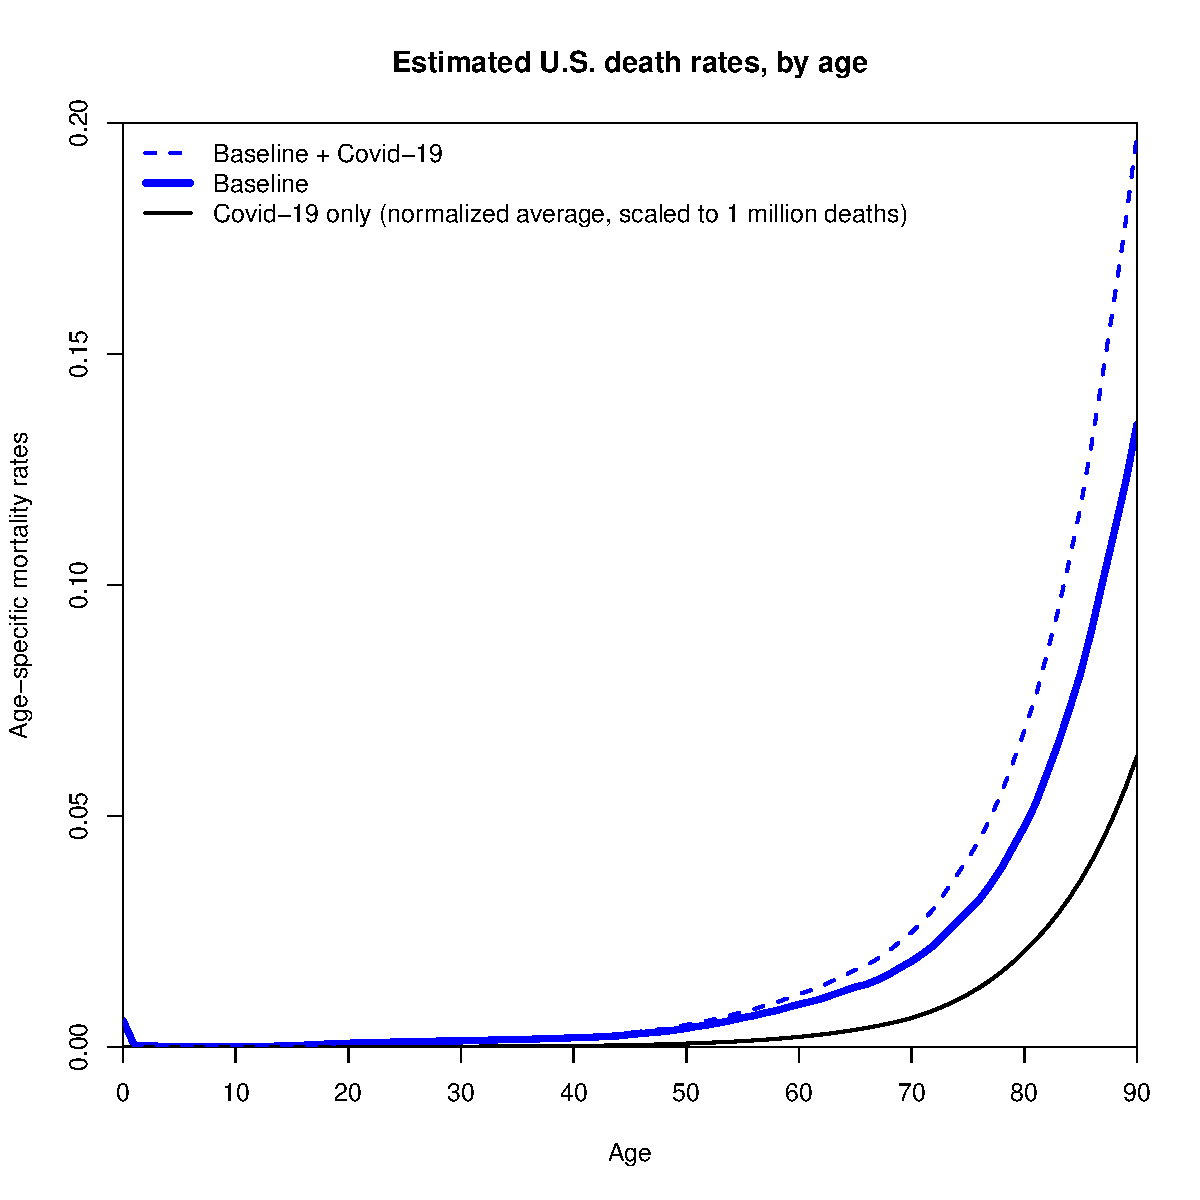
\includegraphics[width=.8\linewidth]{fig3_us_rates}
\caption{Estimated age-specific mortality in the United States in 2020
  for the scenario of 1 million additional Covid-19 deaths. Baseline
  mortality in 2020 is assumed to equal that of 2017. Covid-19
  mortality is estimated by averaging the normalized death rates in
  Figure \ref{fig:asmr}(b), then multiplying these average rates to
  result in 1 million additional deaths using the U.S. population age
  structure for 2020.}
\label{fig:baseline}
\end{figure}


\section*{Loss of remaining life}

Whereas period life expectancy in an epidemic year tells us how long a
person would live if they were to experience an epidemic every year of
their lives, what we would really like to know is how a one-time
epidemic affects the remaining life expectancy of the actual
population.

Based on Social Security Administration projections of cohort
mortality and remaining life expectancy \cite{oact:2020}, we calculate
that the 2020 American population of 330 million people has on average
45.8 years of remaining life expectancy, totaling 14.9 billion
person-years. We calculate, using these same cohort life tables, that
the average person dying of Covid-19 had 11.7 years of remaining life
expectancy, so if the epidemic kills an additional million people, it
will result in a loss of 11.7 million years of remaining life
expectancy. This represents a loss of less than 1/1000th of the
population’s remaining years to live.  Older individuals age 70 to 89,
taking those who die and those who survive together, would on average
lose about .2 years of remaining life, and younger individuals would
lose far less.

How could such an enormous loss of lives produce such a seemingly
small loss of remaining life expectancy? Two factors play a
role. First, even with substantial additional Covid-19 mortality, death will still
be a statistically rare event. Most will survive and they will, if
mortality returns to normal, have many years of life ahead of
them. Second, those who die of Covid-19 are older and have on average
fewer years of remaining life expectancy than the average person (11.7
instead of 45.8).

Our above calculation is specific to the United States and to our
estimated age-pattern of Covid-19, but the small effect of a single
year of epidemic mortality can be seen more generally by extending
Keyfitz's model to a more general formulation of the loss of remaining
life. (See materials and methods \ref{sec:pyl}). This model, like Keyfitz's, also
shows that the effects of an epidemic on loss of remaining
person-years of life, like the effect on life expectancy, scales
roughly proportionately with the magnitude of the epidemic.  We consider a
population that is not growing (``stationary'') experiencing an
epidemic mortality proportional to the baseline age-pattern. An
epidemic that increases mortality by a factor $\Delta$ at all ages
results in a loss of remaining life expectancy equal to
$ H / A \Delta$, where $H$ is Keyfitz’s life table entropy and $A$ is
the mean remaining life expectancy of those alive. For example, if
$\Delta = 1/3$, $H = 0.15$, and $A = 40$ -- roughly the case of the
United States -- this model would predict the share of lost life would
be about 1/800. Unlike our exact calculation above, this model does
not include the older age of death of Covid-19 relative to all-cause mortality,
improvements in mortality implied by using the cohort life expectancy forecast, nor the
particular features of the U.S. age distribution. Nonetheless, such
stylized calculations arrive at a result of the same order of
magnitude.

Both of the above calculations may overstate the loss of remaining
life in that they assigns the remaining life expectancy based only on
age, without taking into account that Covid-19 deaths are
disproportionately occurring among those with compromised health
status. Hanlon et al. \cite{hanlon:2020} estimate that those dying
from Covid-19 have only about one year less of remaining life on
average than those at the same age in the general population, which
would mean that the overstatement is not very large, around 8
percent. On the other hand, our calculations will be an understatement
if the epidemic damages the health of survivors.

The loss of future life seems very small when compared to all of the
years remaining. One way to put the years of remaining life lost from
an epidemic into perspective is to consider it relative to the
person-years lost from mortality in a ``normal'' non-epidemic
year. This calculation accounts for the number and age of deaths from
the epidemic, and weights them by the loss of remaining person years,
comparing the result to the person-years lost in a comparable
non-epidemic year.

\begin{figure*}%[tbhp]
\centering
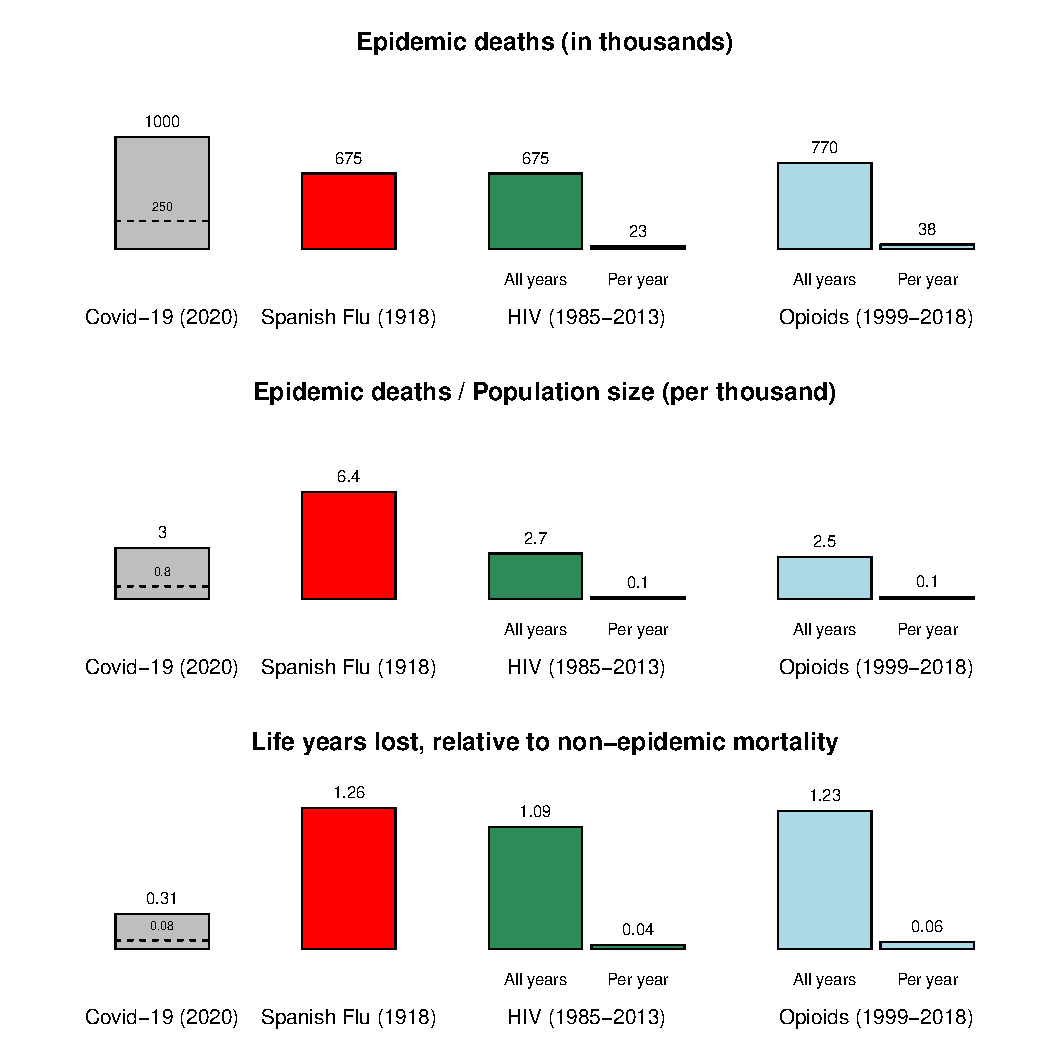
\includegraphics[width=.8\linewidth]{fig4_hiv_plus_new_dash}
\caption{Mortality of Covid-19 scenario compared to past
  U.S. epidemics according to different measures. In the scenario of 1
  million Covid-19 deaths, the virus kills more Americans than past
  epidemics, but when population size is accounted for Spanish Flu is
  more deadly. Taking into account years of remaining life, we
  calculate that the Spanish Flu resulted in even larger losses. The
  scale of the HIV and opioid epidemics were much smaller each year,
  but over decades became comparable to Covid-10 in terms of
  per-capita deaths and Spanish Flu in terms of life-years lost. The
  scenario of 250 thousand Covid-19 deaths is also shown with a dashed
  line.  (Source: authors’ calculations detailed in materials and
  methods \ref{sec:methods_fig4}.)}

\label{fig:epidemics}
\end{figure*}

Using this metric, we estimated the average age of death and computed
the comparative loss of life from Covid-19 relative to the Spanish
Flu, the HIV epidemic, and the recent opioid epidemic according to
three different measurements. For Covid-19 we show scenarios for 1
million and 250 thousand deaths. In the top row of Figure \ref{fig:epidemics}, showing
the counts of deaths, with one million deaths Covid-19 would be the
largest threat we have faced. In the middle row of the figure, which
takes population size into account, Spanish flu emerges as having
produced the largest increase in per capita mortality rates. Taking the age
of those who die into account and their remaining life expectancy, the
bottom panel shows that in terms of lost remaining life expectancy,
our scenario for Covid-19 is much smaller than the Spanish flu. The
dashed lines on the Covid-19 bars show the same calculations based on
250,000 deaths.

The HIV epidemic, which peaked in the 1990s, and opioid overdose
deaths, which continue today, have each over the decades produced
total mortality that is comparable, depending on the metric, to the 1
million death Covid-19 scenario we are considering and even to Spanish
flu. However, on a deaths-per-year basis, they are an order of
magnitude smaller. One million deaths from Covid-19
would confront society in one year, or possibly in just three or four
months, while the deaths we have experienced from HIV or opioid
overdoses occur over the course of decades. This concentration of
epidemic deaths in a short time creates a crisis which overwhelms the
capacities of health care systems, morgues, and mortuaries leading to
triage in hospitals and make-shift storage of bodies such as in an ice
rink in Madrid. The slower-moving epidemics bring other
stresses and anguish, since afflicted individuals suffer for many
years, and the prevalence of those afflicted at any moment is
consequently much higher than for epidemics that kill quickly.

\section*{The valuation of life saved}

We can view these results from a different perspective, comparing the
outcome of an hypothetical uncontrolled U.S. epidemic in 2020 (2 million
deaths \cite{ferguson:2020}) to the far smaller one we may perhaps
achieve with social distancing, which we hypothetically set at
250,000. To ground this number, we note that current projections are
pointing at close to 200,000 deaths by summer's end, with mortality
continuing at some unknown rate afterwards\cite{cdc:2020}. With 2 million deaths, 
period life expectancy at birth for 2020 would have dropped by 5.08 years, 
but with only 250,000 deaths it would drop by only .84 years. An 80 year 
old would lose .40 years of remaining life versus only .05 years. The 
population as a whole would lose about 1/650 of its remaining years
versus only one 1/5100.

In one of the most quoted lines of the Talmud, it is said that whoever
destroys one life, destroys an entire world; and who ever saves one
life is considered to have saved an entire world. Still, policy makers
face the inescapable choice of how many lives to save at what
cost. Federal policy decisions are guided by a substantial literature
in this area. Current estimates for the United States by Viscusi
\cite{viscusi:2018,viscusi:2020} give a single value of \$10 million
to each life regardless of age or alternatively \$500 thousand per
year of life. Using Viscusi’s estimates, which are similar to those
used by the federal government, we can attach a value to a
hypothetical 1.75 million (= 2 million – 250,000) lives saved through
public and private measures taken. Avoiding 1.75 million deaths would
be valued at 17.5 trillion dollars, and saving 20,475,000 person years
of life would be valued at 10.2 trillion dollars. Some other health
economists use substantially lower values around \$125,000 per year of
life \cite{ICER:2020}, which would imply a value of \$2.6 trillion for
avoiding the loss of 20.5 million person years of life.

It is very difficult to evaluate the cost of measures taken to
mitigate the epidemic. The various public transfer programs that have
been enacted are redistributions rather than net social costs,
although they will entail further redistributions as government debt
is serviced in the future. The net societal economic cost of the
public measures taken to mitigate the epidemic is the loss of GDP due
to these measures. Estimating the net cost is an active area of work
\cite{correia:2020,eichenbaum:2020}. Early downward revisions of GDP
forecasts for 2020 by the Congressional Budget Office \cite{cbo:2020}
project about 8\%  less output
than expected (-6\% in 2020 rather than the +2\% projected before
the epidemic), a loss of about \$1.6 trillion. Not all of this decline can be
attributed to societal choices to slow the spread of the virus,
because the economy would also suffer -- perhaps even more -- if the
virus were uncontrolled. But even if we assign all of the drop in GDP
to measures taken to save lives, the economic costs of the actions
society has taken appear to be appropriate for the scale of the
crisis.

\section*{Conclusion}

With a hypothetical one million Covid-19 deaths, it is possible to
portray the epidemic as unimaginably large -- the biggest killer in
American history -- or small, reducing our remaining life
by less than 1 part in 1,000. However, when the loss of
life is put into comparative perspective, we see that the scale of an
epidemic with a million deaths would be as large as the recent opioid
and HIV crises but much smaller than the Spanish flu. The 1918
epidemic killed more people relative to population size, and it also
caused a much greater loss of remaining life expectancy because those
who died were so young.

As a society, we are and we should be making major and costly efforts
to reduce mortality. The anticipated economic costs appear
appropriate, or perhaps low, when compared to the statistical value of
lives that may be saved.

The death toll of Covid-19 is a terrible thing, both for those who
lose their lives and for their family, friends, colleagues and all
whom their lives touched. Those are real individuals, not the abstract
statistics presented here. But the population perspective helps us to
place this tragedy in a broader context. As we put our efforts into
reducing the impact of the epidemic, it is important to know that we
as a society have been through such mortality crises before.


\matmethods{

Data and computer code for replication are available at
\url{https://github.com/josh-goldstein-git/dempersp_covid_mortality}. 
  
\subsection*{Mathematical models}


\subsubsection*{Keyfitz's result for life table entropy}
\label{sec:keyfitz}
Life expectancy at age 0 is computed as the sum of expected person years of
survival of a new born:
$$
e(0) = \int_0^\omega \ell(x) \, dx
$$

Survival $\ell(x)$ is given in terms of the hazard of death $m(a)$ as 
\begin{equation}
  \ell(x) = e^{-\int_0^x m(a) \,da}
  \label{lx_def.eq}
\end{equation}

A populating subject to a new cause of mortality that increases death rates at all ages by
$\Delta$, such that $m(x |\Delta)$ = $m(x) (1 + \Delta)$ will have life expectancy given by
$$
e(0|\Delta) = \int \ell(x)^{1+\Delta} \, dx
$$

Differentiating the logarithm of life expectancy with respect to $\Delta$,
$$
{d \log e(0|\Delta) \over d\Delta} =
{\int \log{\ell(x)}   \ell(x)^{1+\Delta} \, dx \over
  \int \log{\ell(x)}^{1+\Delta} \, dx}
$$
At $\Delta = 0$, this simplifies to
$$
\left.{d \log e(0|\Delta) \over d\Delta}\right|_{\Delta = 0} = {\int \log{\ell(x)}   \ell(x) \, dx \over e(0)}.
$$
Keyfitz defines $H$ as
${-\int \log{\ell(x)} \ell(x) \, dx / e(0)}$. Some further
manipulation gives us the form for $H$ in terms of remaining life
expectancy:
\begin{equation}
  \label{H.eq}
H = {\int d(x)   e(x) \, dx \over e(0)}.
\end{equation}



\subsubsection*{A new result for person years lost}

\label{sec:pyl}
Assume the population is stationary with age structure $c(x) = \ell(x)
/ e(0)$ and that an epidemic raises mortality at all ages by the same
factor $(1 + \Delta)$.

If mortality increases suddenly by a factor of $1 + \Delta$ at all
ages, then, deaths will also increase by the same factor, since in the
immediate term the population exposed to risk will be the same. If
mortality recovers  back to its original level after the epidemic,
then life expectancy of the survivors will remain unchanged, but there
will be fewer survivors.  This means that the total person years of
life left in the population $\theta$ will be 
$$
\theta(\Delta) = B \int \left[\ell(x) - \Delta d(x)\right] e(x) \, dx,
$$
where $B\left[\ell(x) -\Delta d(x)\right]$ is the count of individuals
aged $x$ after the epidemic.

The approximate proportional change in $\theta$ from an epidemic is
then 
$$
-\left.{d \log \theta_0(\Delta) \over d \Delta}\right|_{\Delta = 0} =  
{\int d(x) e(x) \, dx \over \int \ell(x) e(x) \, dx} = {H \over A}
$$
In this result, $H$ is Keyfitz's entropy, defined in (\ref{H.eq}) 
and $A$ is the mean age of the stationary population
$$
A = {\int x \ell(x)\,dx \over e(0)}.
$$

In the United States, $H$ is about 0.15 and $A$ is about 40. If an
epidemic produced an increase of 1/3 in mortality at all ages, 
($\Delta = 1/3$), this would cause a loss of life equal
to $(1/3)(.15)/40 = 1/800$ of the remaining person-years of life of
the population.


\subsection*{Additional methods and data sources}
\subsubsection*{Epidemic mortality rate estimation}
\label{sec:rate}
Covid-19 mortality age-shares for Figure 1 were
calculated using both the age-distribution of Covid-19 attributed
deaths and the age-structure of the population.  Normalization enables
comparison of the age-structure of mortality from populations with
different levels of the epidemic. Normalized rates were calculated by
dividing the unnormalized rates by their sum over all ages, for each
country separately.  Prior to normalization, we adjust for the
population age structure in the open interval aged $80+$ using
indirect standardization.

\subsubsection*{Indirect standardization of open age interval}
\label{sec:indirect}
For indirect standardization, we used the 2017 period both-sex
mortality from the United States as the standard mortality schedule
$M^s_x$ by single years of age $x = 0, \ldots, 99$. We then defined
the share of each population $k$ at each age 80-99, $c_{x,k}$ such that $1
= \sum_{x = 80}^{99} c_{x,k}$, letting the shares for the United
States age structure be the reference age-structure, $c_{x,R}$. The adjustment factor for population $k$
was defined as 
$$
{\sum_x c_{x,R} M^s_x \over
  \sum_x c_{x,k} M^s_x}
$$
The adjustment factors (shown below) were multiplied by the observed  age-specific mortality
rate from Covid-19 for the open interval age $80+$.
\begin{table}[h]
  \centering
  \caption{Adjustment factors used for open age interval}
\begin{tabular}{rrrrrrrr}
France & USA  & England & Spain & Italy & Germany & Korea & Wuhan \\
  \midrule
  0.997 & 1.000 & 1.036 & 1.051 & 1.067 & 1.098 & 1.160 & 1.162 \\
\bottomrule
\end{tabular}
\end{table}

\subsubsection*{Additional information for Figure 1} The average normalized rate is calculated as the arithmetic mean
across countries of the normalized age-specific mortality rates.  The
exponential curve shown in Figure 1(b) is a Gompertz hazard curve with
exponential rate $b = 0.11$, with the level set so that it will intersect
the average normalized rate at age group 70-79.


\subsubsection*{Additional information for Figure 4}
\label{sec:methods_fig4}

We define Annual Mortality Equivalents of the loss of remaining life
expectancy as 
\begin{equation}
AME = {\int D^*(x) e(x) \,dx \over \int D(x) e(x) \,dx},
\end{equation}
where $D^*(x)$ is the number of deaths at age $x$ from a singular mortality event
like an epidemic and $D(x)$ is the number of deaths that would have
been expected in a ``normal'' year. This definition assumes that there
is no difference in the functions of remaining life expectancy by age
but allows for the case when an epidemic has a different age pattern
of deaths.

We can approximate the denominator by expanding $e(x)$ around $x =
A_D = \int x D(x) \,dx / \int D(x)\,dx$, such that $e(x) \approx
e(A_D) + (A_D - x) e'(A_d)$. The second term sums to zero when
integrated against $D(x)$, giving us the approximation
\begin{equation}
  \int D(x) e(x) \,dx \approx  e(A_D) \cdot \int D(x) \, dx.
\end{equation}
Applying the same method to the numerator around $x = A^*_D$ gives

\begin{equation}
  AME = {\int D^*(x) \,dx \over \int D(x) \, dx} \cdot {e(A^*_D) \over e(A_D)}
\end{equation}

This approximation was used for Figure 4 for all of the epidemics
considered, in order to enhance comparability by use of a single
method.

\begin{table}[h]%[tbhp]
  \tiny
\centering
\caption{Parameters used to calculate main text Figure
  4}
\label{tbl:params}

\begin{tabular}{l|rrr|rrr}

  &   \multicolumn{3}{c|}{Epidemic} &  \multicolumn{3}{c}{All-cause} \\
\midrule
 & Deaths & $\bar{x}_e$    &  $e(\bar{x}_e)$ & Reference & Deaths &
                                                                 $e(\bar{x})$
                                                                 \\
  & (1,000s)       &      &           & year & (millions) &  \\     
\midrule
  Spanish flu & 675 & 30 & 38.8 & 1920 (1933) & 1.4 & 15.1 \\
  HIV         & 675 & 40 & 38.0 & 1990        & 2.1 & 11.0 \\
  Opioid &      770 & 42 & 38.8 & 2010        & 2.5 & 9.8 \\
  Covid-19 &    1,000 (250) & 80 & 9.6 & 2017        & 3.0 & 10.2 \\
\bottomrule
\end{tabular}
\normalsize

\addtabletext{Notes: Covid-19 deaths are given for two
scenarios. $\bar{x}_e$ is the mean age of death from each epidemic. $e(\bar{x}_e)$ is the years of remaining life for those
dying from each epidemic. Reference year for Spanish flu uses number of
deaths from 1920 combined with life table from 1933, the first year
national life tables are available to us.  Remaining ``All-cause''
life expectancy $e(\bar{x})$ is calculated as life
  expectancy at average age of death in period life table of reference
  year. Reference years 1990 and 2010 include low-level epidemic
  mortality. The remaining life expectancy at average age of Covid-19
  death differs from value reported in main text in order to use same
  method for different epidemics.}
\end{table}



\subsubsection*{Data Sources for Figure 4}

\paragraph{HIV/AIDS}

    Count of deaths \cite{cdc:2016}. The mean age of HIV-caused death was estimated by tabulating all HIV
deaths from 1979 to 1998 in 5-year age groups and computing the mean
age assuming average deaths in mid-interval. Authors' calculation from
CDC wonder.



\paragraph{Opioid overdoses}
  
Total deaths calculated by authors from data available at \cite{nida:2020}.
The mean age of death for opioid overdoses was computed from CDC
Wonder data tabulated by \cite{kff:2020}.

\paragraph{Spanish Influenza}

  ``The number of deaths was estimated to be at least 50 million worldwide with about 675,000 occurring in the United States.''
  CDC \cite{cdc:2019}.  
The mean age of death was estimated from distributions graphed in Gagnon et al. \cite{gagnon:2013}.


}

%% \setcounter{section}{\Alph}
\appendix

\showmatmethods{} % Display the Materials and Methods section
\acknow{We received helpful comments on this work from
seminar participants in the Department of Demography. Magali Barbieri
helped us find the relevant data for Europe. Yi Zhou helped with the
Chinese data. Peter Choi sent us data for S. Korea. Sam Preston, John
Wilmoth, Barry Schwartz and two anonymous referees provided valuable
suggestions on earlier drafts. Casey Breen helped make the replication
code readable and reproducible. We thank them all. Goldstein is
supported by a grant from the National Institute of Aging R01AG058940.
Both authors are supported by the UC Berkeley Center on the Economics
and Demography of Aging (National Institute of Aging 5P30AG012839),
and the Berkeley Population Center (National Institute for Child
Health and Human Development P2CHD072964).}

\showacknow{} % Display the acknowledgments section

% % Bibliography
%% \bibliographystyle{pnas-new}
\bibliography{DemPersp}
\end{document}


% LocalWords:  Covid
